In this section, we present the results from our simulations experimenting performance impact of executing memory intensive kernels in host processor (host) and PIM execution unit (PIM). Figure~\ref{fig:expr:pim}(a) shows overall performance achievement of Host and PIM cores in terms of Instruction per Cycle (IPC) for all HPC kernels under study. The horizontal bars represent IPC counts for Host and PIM cores whereas the \textit{X} axis lists the benchmarks. The results show that, two kernels from application SimpleMOC and XSBench achieves slightly better performance (2.1\% and 10.3\% speed-up, respectively) when executed on PIM core. Lulesh, RSBench, MiniAMR and Quicksilver kernels' performance deteriorates by 17.2\%, 5.2\%, 16.2\% and 17.24\%, respectively; in comparison to the host core.  Pathfinder's kernels performs the worst suffering a 126.9\% degradation.     


\begin{figure}[!t]
 \centering
  %\vspace*{-2.em}

   \subfloat[IPC.\label{subfig-2:cades}]{
    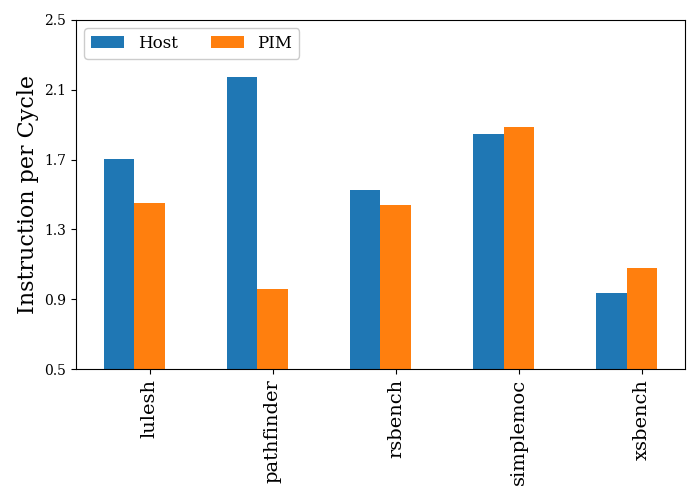
\includegraphics[width=1\linewidth,scale=1.0,keepaspectratio]{MEMSYS22/figures/ipc.png}
  }
  
  \subfloat[MPKI.\label{subfig-2:dgx}]{
    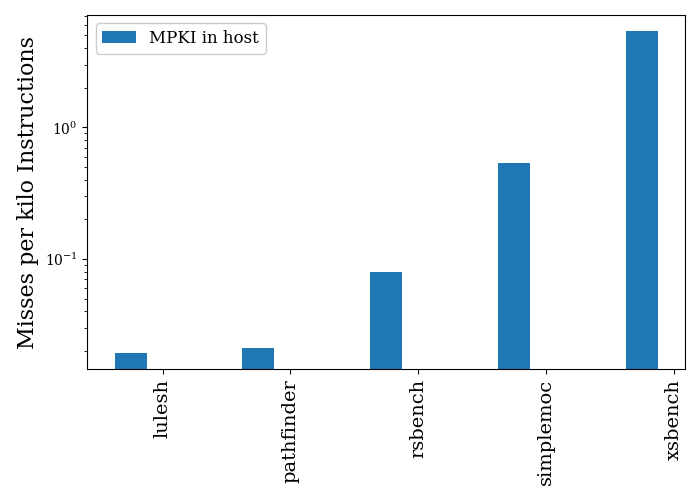
\includegraphics[width=1\linewidth,scale=1.0,keepaspectratio]{MEMSYS22/figures/mpki.png}
  }
  
   \subfloat[LFMR.\label{subfig-2:crusher}]{
    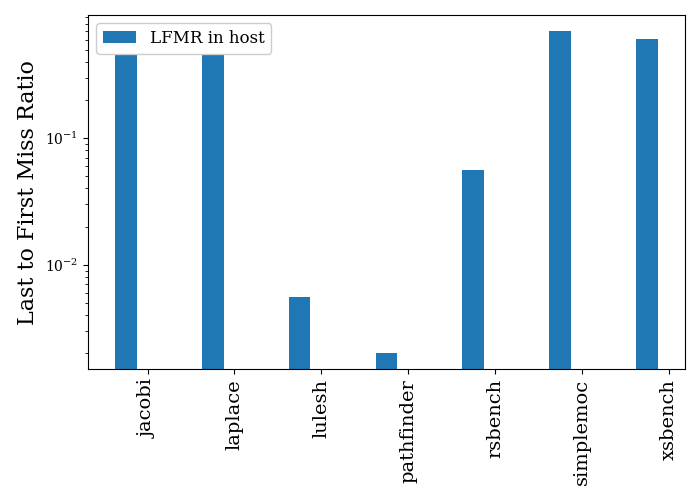
\includegraphics[width=1\linewidth,scale=1.0,keepaspectratio]{MEMSYS22/figures/lfmr.png}
  }
  
   \vspace{-.05in}
   \caption{ Performance impact of HPC kernel executing on PIM core in comparison to the Host core. (a) Performance variation in terms of Instruction Per Cycle (IPC) for Host and PIM cores. (b) L3 Misses Per Kilo Instruction (MPKI) for all Kernels in host core (c) Last to First Miss Ratio (LFMR) on host core for kernels under analysis.}   
 \vspace{-.3in}
 \label{fig:expr:pim}
 \vspace{-1em}
\end{figure}

To investigate the variation in performance, we analyze L3 \textit{Misses Per Kilo Instructions} (MPKI) for each kernel in the host core, presented in Figure~\ref{fig:expr:pim}(b), where \textit{Y} axis lists the MPKI values in logarithmic scale and \textit{X} axis lists the name of the applications. The chart shows that the MPKI values for application kernels range from 0.011 (MiniAMR) to 4.65 (XSBench). SimpleMOC and XSBench that perform better in PIM core has the highest MPKI values among the kernels under analysis. We further analyze \textit{Last to First Miss Ratio (LFMR)} which corresponds to the miss ratio between L3 cache misses and L1 cache misses, presented in  Figure~\ref{fig:expr:pim}(c). LFMR effectively indicates the efficiency of the cache hierarchy. For the HPC kernels under study, LFMR ranges from 0.002 (Pathfinder) to 0.7 (SimpleMOC). An interesting observation from this is, although miniAMR has lower MPKI (0.011) than Pathfinder (0.021), but with higher LFMR it performs relatively better on the PIM core.   




%It indicates that performance improvement in the PIM core is related with     







%
%\begin{figure}[t!]
%\hspace*{-9.5cm}
%\centering
%\includegraphics[width=\textwidth, height=60mm]{figure/Set1.pdf}
%%\caption{ST-1.2 Configuration (floating point benchmarks): Speedup ranges from 0\% (tonto) to 7.4\% (milc), and it is 2.7\% on average.}
%\label{fig:Set1}
%\end{figure}
%
%
%\begin{figure}[htbp]
%  
%\centering
%\includegraphics[width=\textwidth, height=60mm]{figure/Set2.pdf}
%%\caption{ST-1.2 Configuration (floating point benchmarks): Speedup ranges from 0\% (tonto) to 7.4\% (milc), and it is 2.7\% on average.}
%\label{fig:Set2}
%\end{figure}
%
%
%\begin{figure*}[t!]
%\centering
%\includegraphics[width=\textwidth, height=60mm]{figure/Set3.pdf}
%%\caption{ST-1.2 Configuration (floating point benchmarks): Speedup ranges from 0\% (tonto) to 7.4\% (milc), and it is 2.7\% on average.}
%\label{fig:Set3}
%\end{figure*}
%
%%\vspace{5cm}
%\newpage
%
%\begin{figure}[H]
%\centering
%\includegraphics[width=\textwidth, height=60mm]{figure/Set4.pdf}
%%\caption{ST-1.2 Configuration (floating point benchmarks): Speedup ranges from 0\% (tonto) to 7.4\% (milc), and it is 2.7\% on average.}
%\label{fig:Set4}
%\end{figure}








